\begin{frame}[parent={cmap:jabuti-gui},hasnext=true,hasprev=true]
\frametitle{Main functionalities}
\framesubtitle{Test Case Menu}
\label{concept:test-case-menu}

\begin{block}{Test case}
The \highlight{Test Case} menu provides options for test set manipulation and
report generation.
\end{block}

\begin{block}{Demo}
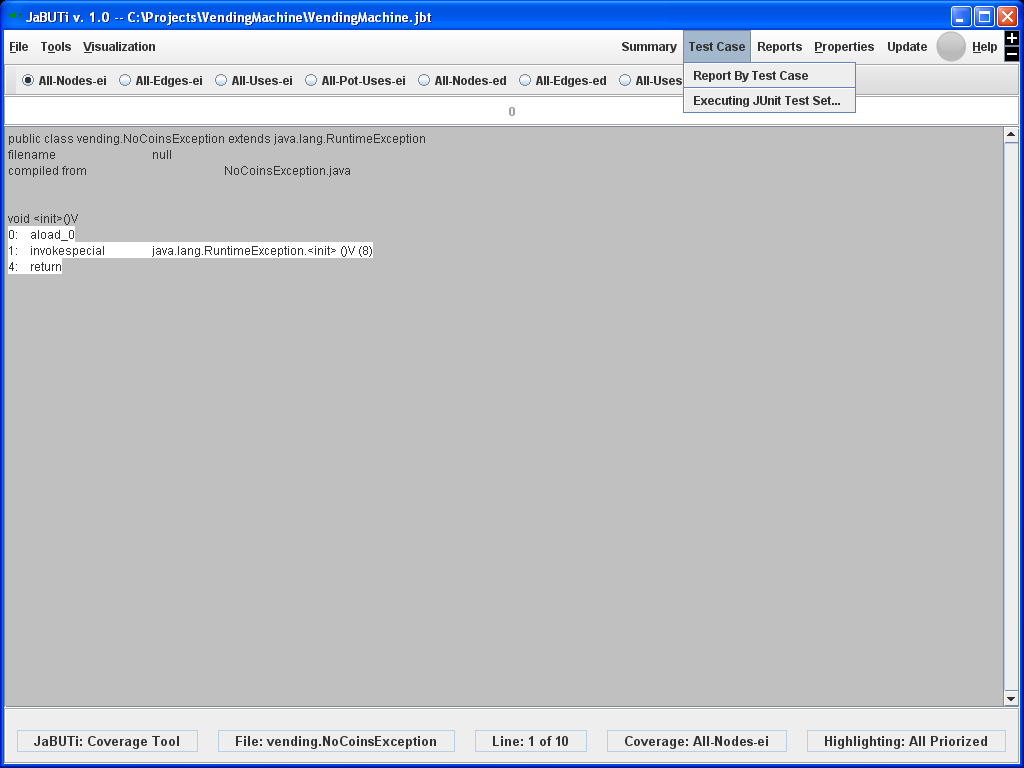
\includegraphics[width=\textwidth,clip]{resources/JaBUTi/JaBUTi-GUI/JaBUTi-GUI-TestCase/JaBUTi-GUI-TestCase}
\end{block}
\end{frame}



\begin{frame}
\frametitle{Main functionalities}
\framesubtitle{Test Case Menu}
\label{concept:report-by-test-case}

\begin{block}{Report By Test Case}
\highlight{Report By Test Case} option shows the coverage information with
respect to the current selected test criterion, for each individual test case,
considering all class under testing, and also allows to enable/disable and
delete/undelete test cases.
\end{block}

\begin{block}{Demo}
\insertmovie{JaBUTi/JaBUTi-GUI/JaBUTi-GUI-TestCase-ReportByTestCase/JaBUTi-GUI-TestCase-ReportByTestCase}
\end{block}
\end{frame}



\begin{frame}
\frametitle{Main functionalities}
\framesubtitle{Test Case Menu}
\label{concept:importing-from-junit}

\begin{block}{Importing from JUnit}
\highlight{Importing from JUnit} option allows to import a test set generated
according to the JUnit framework.
\end{block}

\begin{block}{Demo}
\insertmovie{JaBUTi/JaBUTi-GUI/JaBUTi-GUI-TestCase-ExecutingJUnitTestSet/JaBUTi-GUI-TestCase-ExecutingJUnitTestSet}
\end{block}
\end{frame}
